% !TeX root = ../main.tex

\chapter{Device fabrication of silicon nitride ring resonators}\label{chap:4}

Different from fabrication of silicon photonic devices based silicon-on-insulator (SOI) wafers, which is CMOS-compatible and widely used in the laboratory and semiconductor industry, to fabricate integrated silicon nitride device, in particular high \textit{Q}-factor ring resonators realizing four wave mixing, is still challenging.
Collaborating with Yokoyama Lab in Kyushu University, we perform the subtractive fabrication of silicon nitride ring resonators as well as other optical devices. 

%\section{Subtractive fabrication process}

The subtractive process refers to the subtraction of unnecessary parts after the patterning, differing from the lift-off or damascence processes. For optical devices, it challenges the etching recipe to achieve less roughness on the sidewalls. 
% abrication of waveguide is widely perform in a variety of material platforms, including silicon nitride.
The previous work using similar fabrication processes reported silicon nitride ring resonators with \textit{Q}-factor up to \num{5.2d4}. The measured loss of waveguides is 2.9 dB/cm \cite{Cheng2017b}. 

\begin{figure}
	\centering
	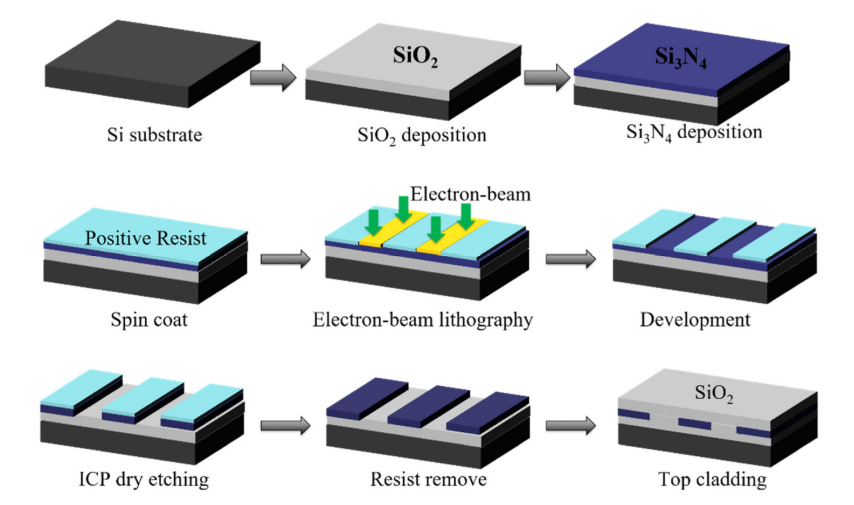
\includegraphics[width=1.0\linewidth]{imgs/png/fab-flow}
	\mycaption{Schematic process flow of the subtractive process from Reference \cite{Cheng2017b}}{The process used in this thesis is identical.}
	\label{fig:fab-flow}
\end{figure}

The schematic process flow of the subtractive process is illustrated in \autoref{fig:fab-flow}. First, the silicon dioxide film is deposited on a 4-inch silicon substrate using the TEOS  (tetraethyl orthosilicate) source.
An alternative method is using a thermal oxidized silicon wafer directly. The target thickness of silicon dioxide layter is greater than 2 \um to create enough buffer between the silicon nitride film and the silicon substrate. 
Next is silicon nitride film deposition using chemical vapor deposition methods. Following electron beam (EB) lithography patternning, the silicon nitride layer is etched with inductively coupled plasma reactive-ion etching (ICP RIE) technique. After the resist removal, another layer of silica is cladded. Finally, the chip is cut to couple the light from the edge. 

The details of each step will be expanded in the following contents.

\section{Film deposition}

Low pressure CVD (LP-CVD) is a traditional method to deposit silicon nitride from the vapor source by the decomposition of chemicals on the surface.  
Stoichiometric silicon nitride can be obtained by controlling and optimizing the ratio of silicon and nitrogen sources. 
The precursor of silicon is usually silane (\ce{SiH4}) or chloride silane gases, such as dichlorosilane (DCS, \ce{SiH2Cl2}). And the ammonia gas (\ce{NH3}) plays the role of nitrogen source. 
\begin{align*}
    \ce{3SiH4(g) + 4NH3(g) &-> Si3N4(s) + 12H2(g)} \\
    \ce{3SiH2Cl2(g) + 4NH3(g) &-> Si3N4(s) + 6HCl(g) + 6H2(g)}
\end{align*}

Considering the toxic gases used in LP-CVD, an alternative approach is to use modern plasma-enhanced CVD (PE-CVD) with liquid source, which has faster growing rate and lower reaction temperature. 

% Although the silicon nitride waveguides deposited by LP-CVD method are mainly reported, it is necessary to figure out the CVD method dependence of film properties, especially the refractive index. 

To compare the CVD method dependence of film properties, especially the refractive index, in our research, three different CVD facilities---LP-CVD, PE-CVD and liquid source CVD (LS-CVD) are exploited with corresponding recipes.

Compared with commercial silicon nitride on insulator wafers deposited using LP-CVD,
the details of PE-CVD and LS-CVD recipes are listed in \autoref{tab:cvd}. It is apparent from the data that LS-CVD has the fastest rate 23 nm/min, and lowest reaction temperature. In addition, during our experiments, although the flow rate of SN-2 source changes the film growing rate, it does not effect the film stoichiometry and optical properties. 
% This is different from PE-CVD facility used in this research, which can be also used to produce silicon-rich or nitrogen-rich films as controlling the gas ratio.
It is also worth to mention that all the wafer deposited with above three recipes shows no cracks during our fabrication, suggesting low tensile in these silicon nitride films.

\begin{table}
\centering
\mycaption{Recipes of CVD methods used in this research}{In the case of PE-CVD and LS-CVD, upper electrode and lower electrode are set at different temperature. RF power refers to radio frequency power used to excite the precursor gasses.}
\label{tab:cvd}
\begin{tabular}{cccc}
%\hline
              & LP-CVD                            & PE-CVD                                                                                  & LS-CVD                                                                                  \\ \hline
Facility      & -                                 & SAMCO PD-220NL                                                                          & SMACO PD-100ST                                                                          \\ \hline
Source        & DCS:\ce{NH3}:\ce{N2}                        & \begin{tabular}[c]{@{}c@{}}\ce{SiH4}:\ce{NH3}:\ce{N2}\\ =6:5:189 sccm\end{tabular}                     & \begin{tabular}[c]{@{}c@{}}SN-2:\ce{N2}\\ =0.5:30 sccm\end{tabular}                          \\ \hline
Chamber Temp. & 750\si{\celsius}-800\si{\celsius} & \begin{tabular}[c]{@{}c@{}}upper 150\si{\celsius}\\ lower 350\si{\celsius}\end{tabular} & \begin{tabular}[c]{@{}c@{}}upper 150\si{\celsius}\\ lower 180\si{\celsius}\end{tabular} \\ \hline
RF Power      & -                                 & 40 W                                                                                     & 30 W                                                                                     \\ \hline
Deposition Rate          & -                                 & 15 nm/min                                                                               & 23 nm/min                                                                               \\ \hline
\end{tabular}
\end{table}




\section{Patterning}
The sample used in our experiments are usually in the size of 20 mm $\times$ 20 mm, diced off from a 4-inch wafer. 
All the samples are cleaned several times using acetone solution in a ultrasonic cleaning device for at least 5 min.
Before resist coating, a step of oxygen ashing is helpful to remove the particles over sample surface.

First, a layer of an adhesion promoter, hexamethyldisilazane (HMDS) is coated at 2000 rpm and then baked at 120 \si{\celsius} for 1 min. Next, the positive resist (AR-P 6500, ALLRESIST GmbH) is coated at 1000 rpm and soft-baked at 120 \si{\celsius} for 2 min. The final thickness of resist is around 800 nm to achieve enough thickness during the etching process. The main electron-beam lithography (EBL) machine used in our experiments is ELIONIX ELS-F100 and the beam dose is 3 nA, 0.6 sec/dot. This recipe is fully optimized and has small feature sizes and high accuracy around 10 nm. After the lithography, the sample is developed using \textit{o}-xylene for 1 min. 

% Several EB resists are compared, both negative and positive type. 

\section{ICP etching}

In order to etch the waveguide layer selectively, ICP-RIE (RIE-400iPB, SAMCO Inc.) is used to remove the unmasked section in silicon nitride layer.

Different from previous work \cite{Yusuke2017}, the ICP-RIE facility used in this study is optimized for deep silicon etching. In the key etching step of our recipe, only \ce{CHF3} gas, 6 sccm, is used as well as with argon gas to cleans any residual organic matter over the surface. ICP power is set 50 W, and RF bias power is 20 W.

The etching rate of three kinds of film is listed in \autoref{tab:cvd}. From the data, we can see LS-CVD deposited film has the best selectivity, much higher than LP- and PE-CVD samples. It seems possible that the film density varies from the CVD methods, due to LS-CVD has the fastest growth rate and lowest reaction temperature.

\begin{table}
\mycaption{Etching rate and selectivity of ICP process}{The etching rate is evaluated by step height measured via step profiler.}
\label{tab:icp}
\begin{tabular}{cccc}
%\hline
       & \begin{tabular}[c]{@{}c@{}}Film Etching Rate \\ (nm/min)\end{tabular} & \begin{tabular}[c]{@{}c@{}}Resist Etching Rate\\ (nm/min)\end{tabular} & Selectivity \\ \hline
LP-CVD & 19.20                                                            & 12.76                                                                     & 1.50        \\ \hline
PE-CVD & 23.48                                                            & 14.29                                                                     & 1.64        \\ \hline
LS-CVD & 27.40                                                            & 2.08                                                                      & 13.17       \\ \hline
\end{tabular}
\end{table}

\section{Top oxide cladding}
The final step is cladding another layer of silicon dioxide to increase the coupling efficiency of ring resonators, as a result of lower index contrast. Before film deposition, to remove not only the residual EB resists but also the polymer generated during the plasma etching, 
all the samples are first deeply ashed using normal oxygen recipe in another RIE facility. To reduce the damage of waveguide sidewall, this step is cycled with organic cleaning. 
As same as the buried oxide layer, TEOS source is used to deposit another 2-3 \um top cladding layer with the same LS-CVD facility.

\section{Annealing}

To remove the residual hydrogen in silicon nitride film, an optional step of annealing is necessary. 
Traditionally, annealing process can be performed in different cases, after or during CVD deposition \cite{Luke2013}, after dry etching or after top cladding \cite{Ang2018}. Since the first case requires tensile control during cycled deposition-annealing operation \cite{Luke2013}, in our experiments, annealing before or after top cladding of negatively patterned LS-CVD and PE-CVD sample are merely compared.

To achieve high vacuum during the annealing, we use a tube-type electric furnace. In a high vacuum, the furnace is set first heating gradually  from room temperature to 300 \si{\celsius} for 1 h, then heating to 1000 \si{\celsius} for 3 h, keeping at 1000 \si{\celsius} for 4 h, and cooling down to 300 \si{\celsius} for 5 h, then naturally cooling to room temperature. 

Shown in \autoref{fig:anneal}, there are cracks on both the LS-CVD and PE-CVD samples. In contrast, the negatively patterned samples are free of any cracks but is severely contaminated, which possibly results from the residua in the tube furnace. 
In general, the finding of cracks on the top clad layer shows despite the tensile control over the silicon nitride film, even negative EB resist is used for layout transfer, it is still difficult to annealing the typical TEOS cladded samples with the PE-CVD facility in our fabrication condition.

\begin{figure}
    \centering
    \begin{subfigure}[b]{0.45\textwidth}
    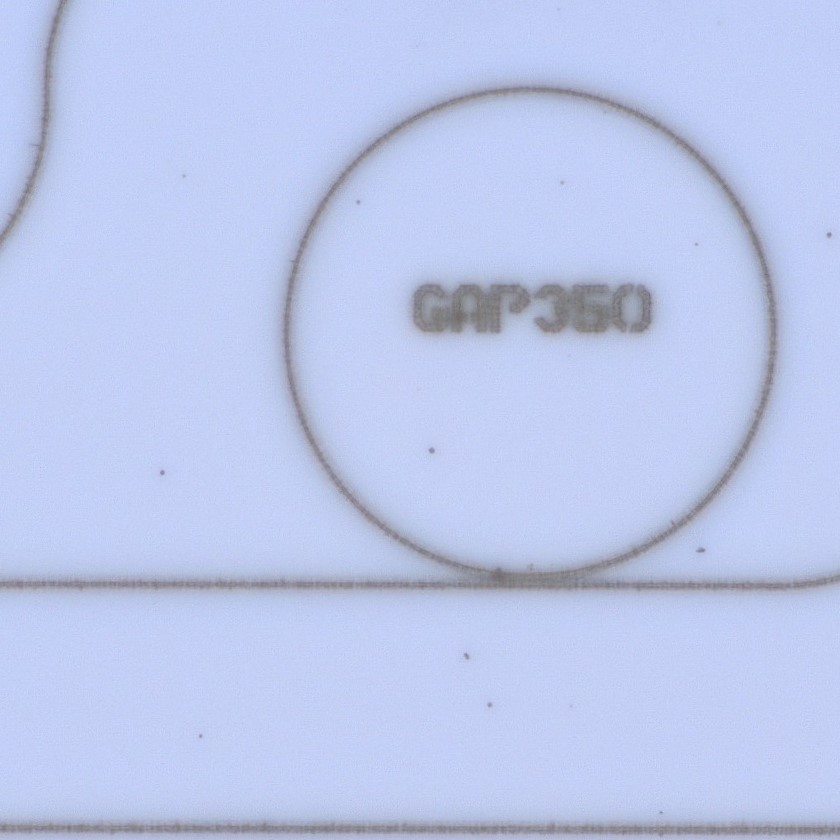
\includegraphics[width=\textwidth]{imgs/jpg/LS_ac}
    \caption{}
    \end{subfigure}
    \begin{subfigure}[b]{0.45\textwidth}
    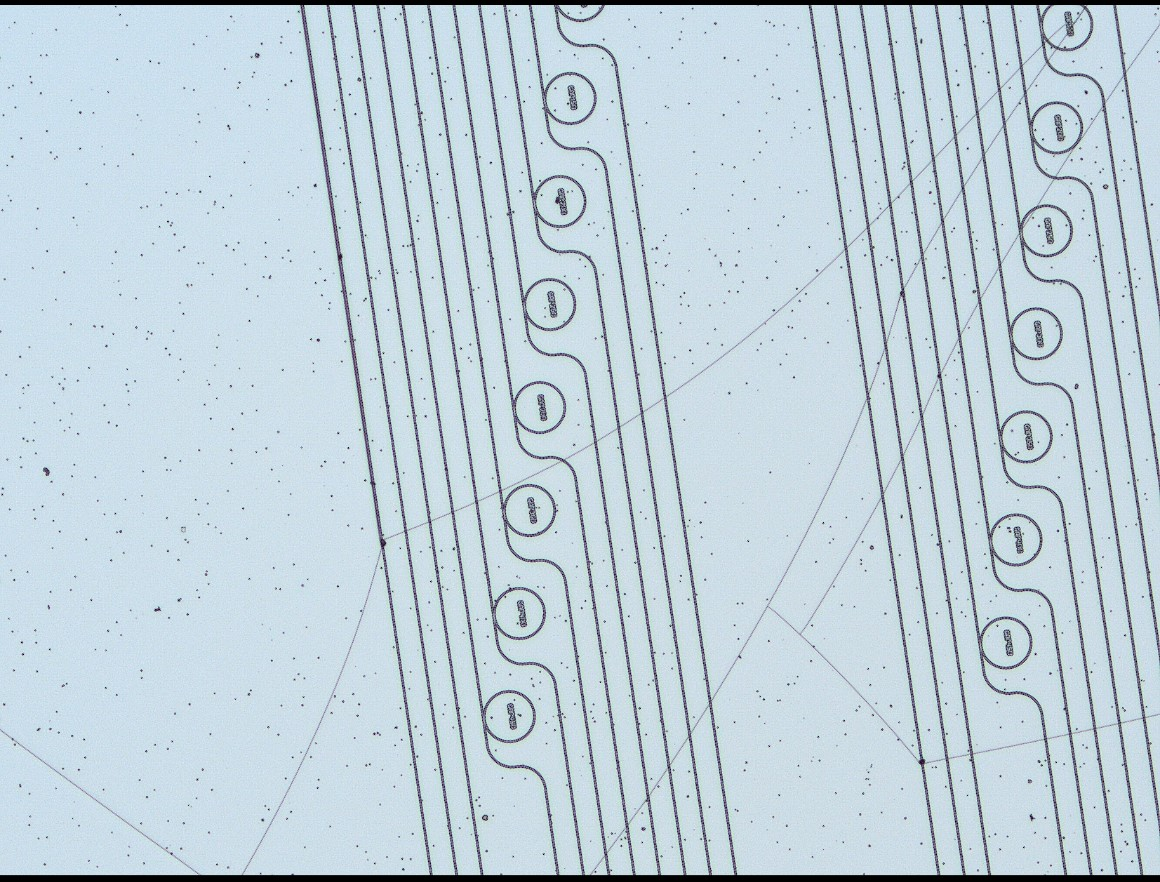
\includegraphics[width=\textwidth]{imgs/jpg/LS_tc}
    \caption{}
    \end{subfigure}    
    \begin{subfigure}[b]{0.45\textwidth}
    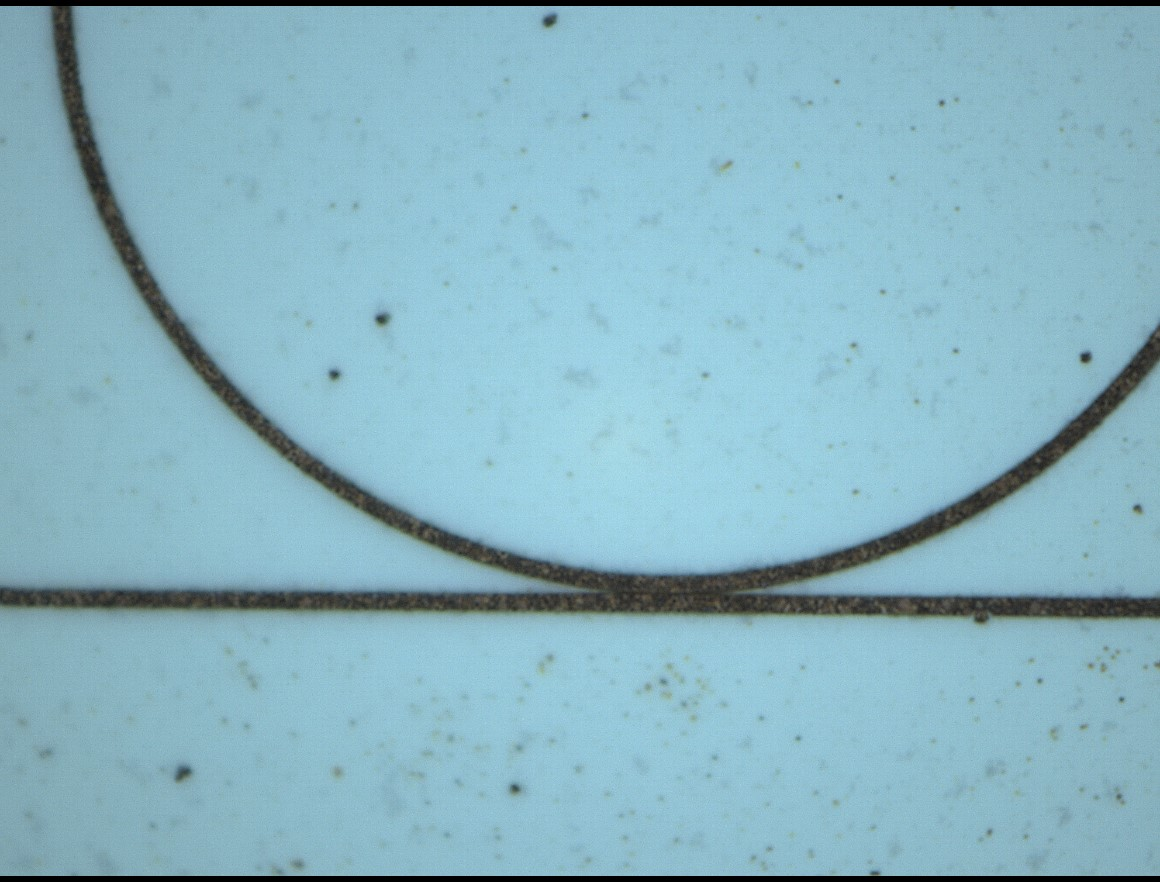
\includegraphics[width=\textwidth]{imgs/jpg/SR_ac}
    \caption{}
    \end{subfigure}
    \begin{subfigure}[b]{0.45\textwidth}
    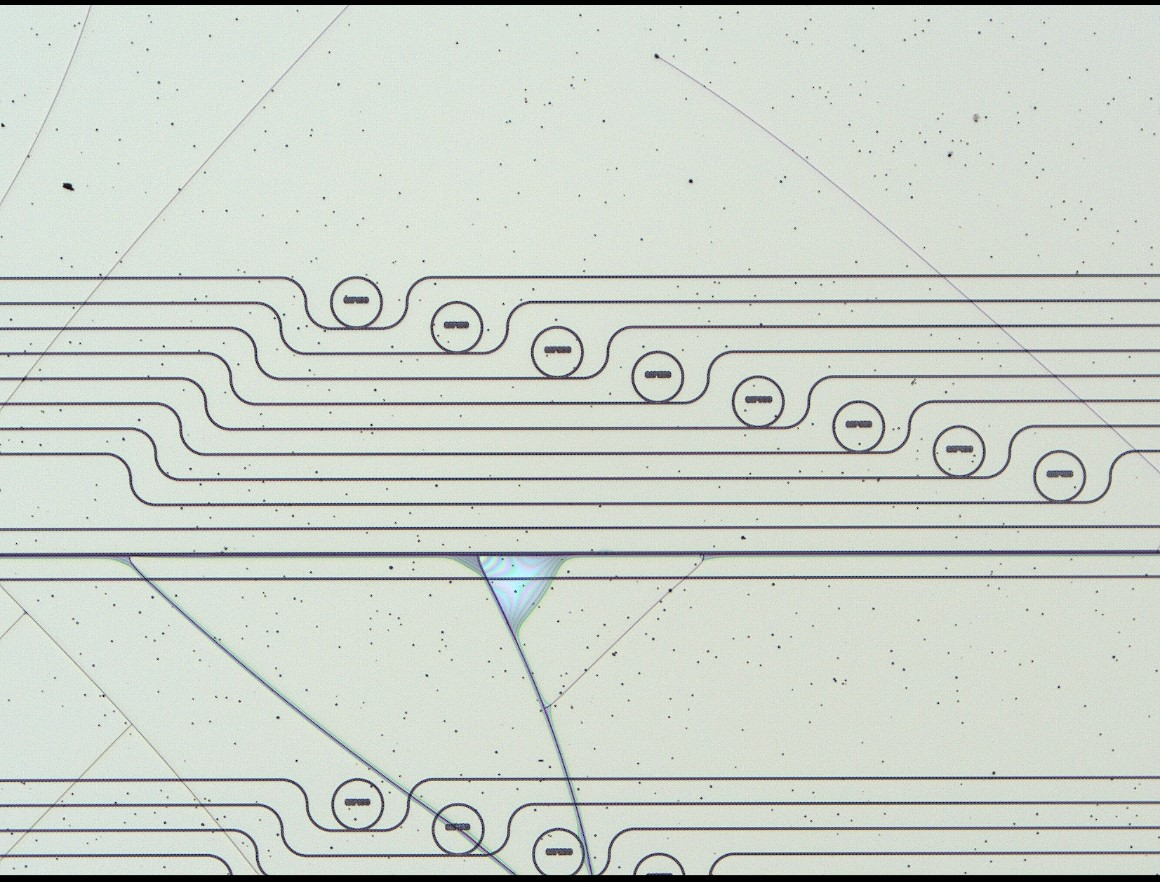
\includegraphics[width=\textwidth]{imgs/jpg/SR_tc}
    \caption{}
    \end{subfigure}
    \mycaption{Laser microscope images of samples after annealing process}{All the sample are annealed under the same circumstance. \textbf{a}. LS-CVD sample without top cladding. \textbf{b}. LS-CVD sample with TEOS top-cladding. \textbf{c}. PE-CVD sample without top cladding. \textbf{d}. PE-CVD sample with TEOS top-cladding. The cracks origin from contamination shown in \textbf{b} and \textbf{d}.}
    \label{fig:anneal}
\end{figure}

\section{Chip dicing}\label{sec:chip-dicing}

The final step of fabrication is to disclose the input and output ports of bus waveguides.
A conventional method is using diamond scribe to define the direction of wafer cleaving, whose accuracy depends on scribe end width.
While in the case of devices with mode convertors, 
to precisely define the input and output ports, the chip dicing is required.

Compared with conventional mechanical dicing,  the laser dicing technique is advantageous at high precision and less damages on the chip edges. The image of laser diced edge is compared with the manually diced one in \autoref{fig:dicing}. Apparently, the chip using laser dicing has smoother edge, which is helpful to reduce the backward scattering during fiber launching.

\begin{figure}
    \centering
	\begin{subfigure}[b]{0.45\textwidth}
		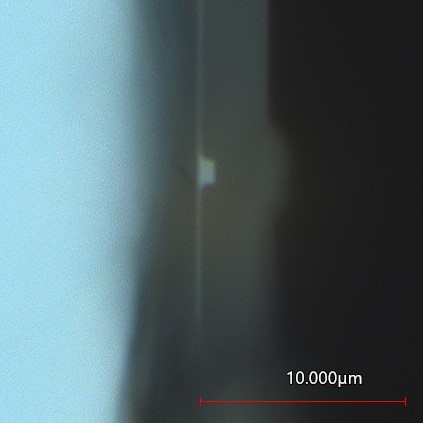
\includegraphics[width=\textwidth]{imgs/jpg/laser}
 		\caption{}
	\end{subfigure}
	\begin{subfigure}[b]{0.45\textwidth}
		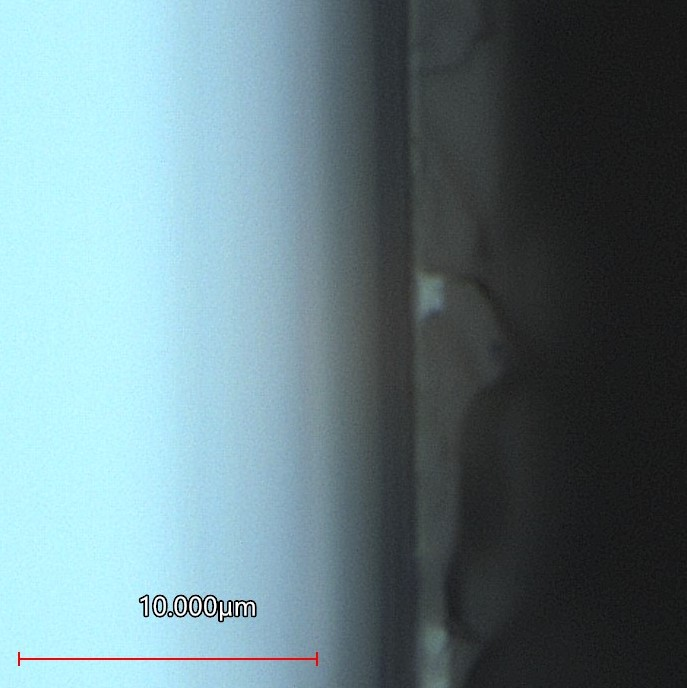
\includegraphics[width=\textwidth]{imgs/jpg/manual_cleav}
 		\caption{}
	\end{subfigure}
    \mycaption{Microscope images of chip edge diced by laser dicing and manually cleaving.}{\textbf{a} Laser diced. \textbf{b} Manually cleaved. The scale in the images is 10 \si{um}.}
    \label{fig:dicing}
\end{figure}

\newpage
\section{Summary}
To summarize the fabrication process used for silicon nitride ring cavities, several problems occur and result in device nonresonance sometimes. First is the cleaning, we found using organic solution is not enough for particle removal before spin coating. A solution can be multiple filtering of electron beam resist. Another problem is film etching. Previous research \cite{Ono2017} studied different etching recipes, which are not covered in this thesis. But due to low recipe reproducibility, fully optimization is still necessary.
Furthermore, the trade-off between film thickness and annealing still exists. An future alternative is using metallic hardmask against the etching plasma and adding deeper trenches around ring resonators to prevent cracking.


